\begin{exercício}{Indutância mútua entre espiras grande e pequena}{exercício2}
    Uma \emph{pequena} espira circular de raio \(a\) se encontra a uma distância \(z \gg a\) acima do centro de uma \emph{grande} espira de raio \(b \gg a\). Os planos das espiras são paralelos e seus centros estão sobre o eixo comum de simetria, como mostra a figura abaixo.
    \begin{center}
        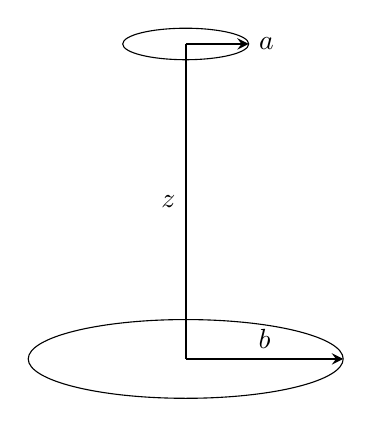
\begin{tikzpicture}
            \draw (0,0) ellipse (2 and 0.5);
            \draw (0,4) ellipse (0.8 and 0.2);
            \draw[thick] (0,0) -- (0,4) node[midway,left] {\(z\)};
            \draw[thick, -stealth] (0,0) -- (2,0) node[midway, above] {\(b\)};
            \draw[thick, -stealth] (0,4) -- (0.8,4) node[right] {\(a\)};
        \end{tikzpicture}
    \end{center}
    \begin{enumerate}[label=(\alph*)]
        \item Suponha que haja uma corrente estacionária \(I\) na espira grande. Qual o fluxo magnético sobre a espira menor? \todo[Considere que a área da espira menor é pequena o suficiente para que o campo seja uniforme sobre ela]
        \item Suponha que haja uma corrente estacionária \(I\) na espira menor. Qual o fluxo magnético sobre a espira maior? \todo[Considere que a espirta menor é pequena o suficiente para que possa ser aproximada por um dipolo dial]
        \item Encontre a indutância múta e confirme que \(M_{21} = M_{12}\). \todo[Recordamos que a indutância mútua entre os objetos \(1\) e \(2\), \(M_{21}\), é definida como a razão entre o fluxo sobre o objeto \(2\) devido ao campo magnético gerado pela corrente \(I_1\) do objeto \(1\), ou seja \(\Phi_{B_{2(1)}} = M_{21}I_1\).]
    \end{enumerate}
\end{exercício}
\begin{proof}[Resolução]

\end{proof}
